\documentclass[12pt,xetex,serif]{beamer}
\mode<presentation>{}
\usepackage{beamerthemeBMlibrary}
\mode<presentation>
\usetheme{Madrid}
\usepackage{multicol}
\begin{document}
	\begin{frame}
		\titlepage
	\end{frame}
	%\begin{frame}
		%\contentsname
		%\tableofcontents
	%\end{frame}
	\begin{frame}{ទ្រឹស្តីសុីនេទិចនៃឧស្ម័នបរិសុទ្ធ}
		\begin{multicols}{2}
			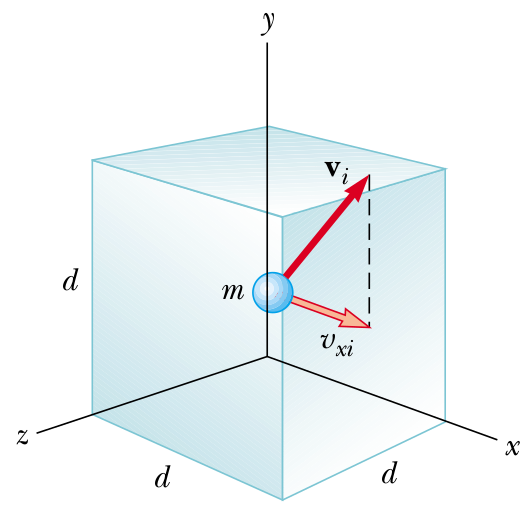
\includegraphics[scale=0.2]{gases1}
			\begin{enumerate}
				\item ម៉ូលេគុលឧស្ម័នធ្វើចលនាឥតឈប់ឈរ និងគ្មានសណ្តាប់ធ្នប់
				\item ទង្គិចរវាងម៉ូលេគុល នឹងម៉ូលេគុល ឬផ្ទៃខាងនៃធុងជាទង្គិចខ្ទាត
				\item ចន្លោះពេលទង្គិចម៉ូលេគុលឧស្ម័នមានចលនាត្រង់ស្មើ(ល្បឿនថេរ)
				\item ថាមពលសុីនេទិចរបស់ម៉ូលេគុលឧស្ម័នអាស្រ័យទៅនឹងសីតុណ្ហភាព
				\item គេចាត់ទុកម៉ូលេគុលឧស្ម័នជាចំណុចរូបធាតុ។
			\end{enumerate}
		\end{multicols}
	\end{frame}
	\begin{frame}{សម្ពាធក្នុងទ្រឹស្តីសុីនេទិចនៃឧស្ម័ន}
			\text{បរិមាណចលនាមុនពេលទង្គិច}\quad $\overrightarrow{p_1}=m\vec{v_1}$\\
			\text{បរិមាណចលនាក្រោយពេលទង្គិច}\quad $\overrightarrow{p_2}=-m\vec{v_2}$
		\begin{center}
			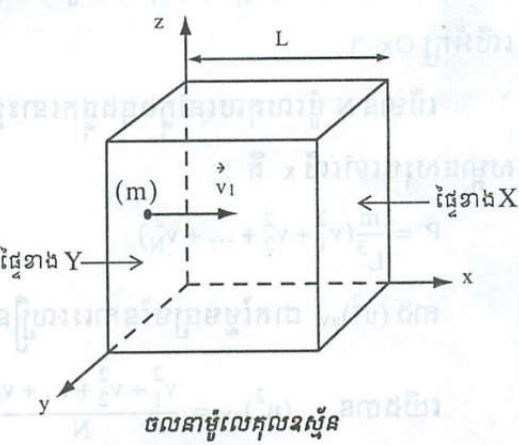
\includegraphics[scale=0.3]{gases2}
		\end{center}
	\end{frame}
    \begin{frame}{\bibname}
    	
    \end{frame}
\end{document}